\begin{frame}
	\maketitle
\end{frame}

\begin{frame}{Introduction}
	The Capacitated Vehicle Routing Problem (\textbf{CVRP}) is a \textcolor{blue}{discrete optimization routing problem} with applications in \textcolor{blue}{logistics optimization} (goods/services delivery).

	\vspace{0.5cm}

	\begin{columns}
		\begin{column}{.35\textwidth}
			\centering
			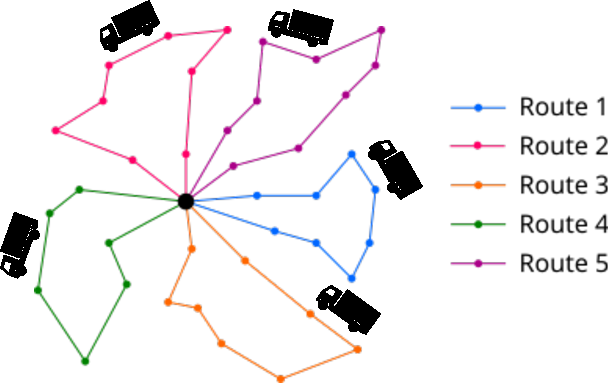
\includegraphics[height=4cm]{Imgs/CVRP-example-without-truck.out.cropped.pdf}
		\end{column}
		\begin{column}{.65\textwidth}
			We are given:
			\begin{itemize}
				\item Customer \textcolor{blue}{locations} within the road network
				\item The \textcolor{blue}{demand} of each customer.
				\item The \textcolor{blue}{vehicle capacity}.
				\item Number of \textcolor{blue}{available trucks}.
			\end{itemize}
			Objective:
			\begin{itemize}
				\item \textcolor{red}{Serve all customers while minimizing the overall routing cost}.
			\end{itemize}
		\end{column}
	\end{columns}

\end{frame}

\begin{frame}{Branch-price-and-cut}
\end{frame}

\begin{frame}{Conclusions}
	Thank, you.

	\cite{jepsen2014}
\end{frame}

\begin{frame}
	\maketitle
\end{frame}
